\chapter{Summary of Chai Commands}
%\begin{figure}[t]
%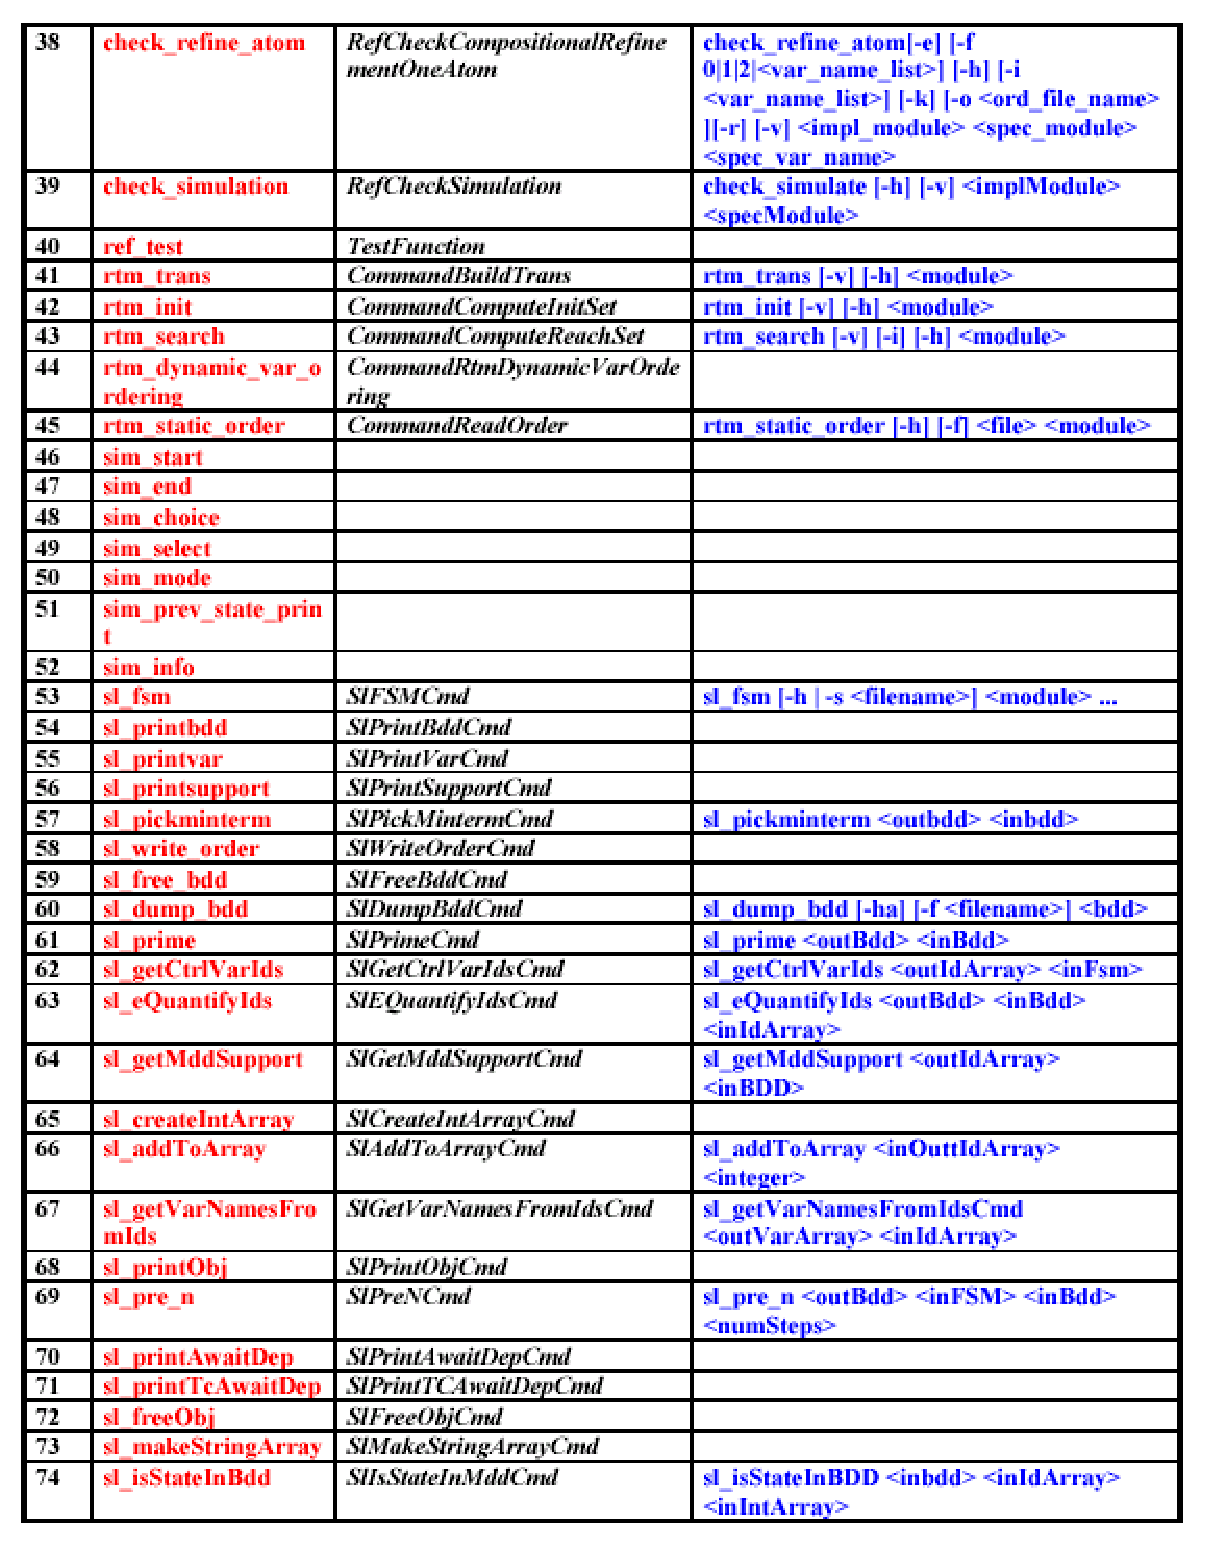
\includegraphics[width=1in,height=2in]{figs/page-2}
%\end{figure}

%\newpage
%%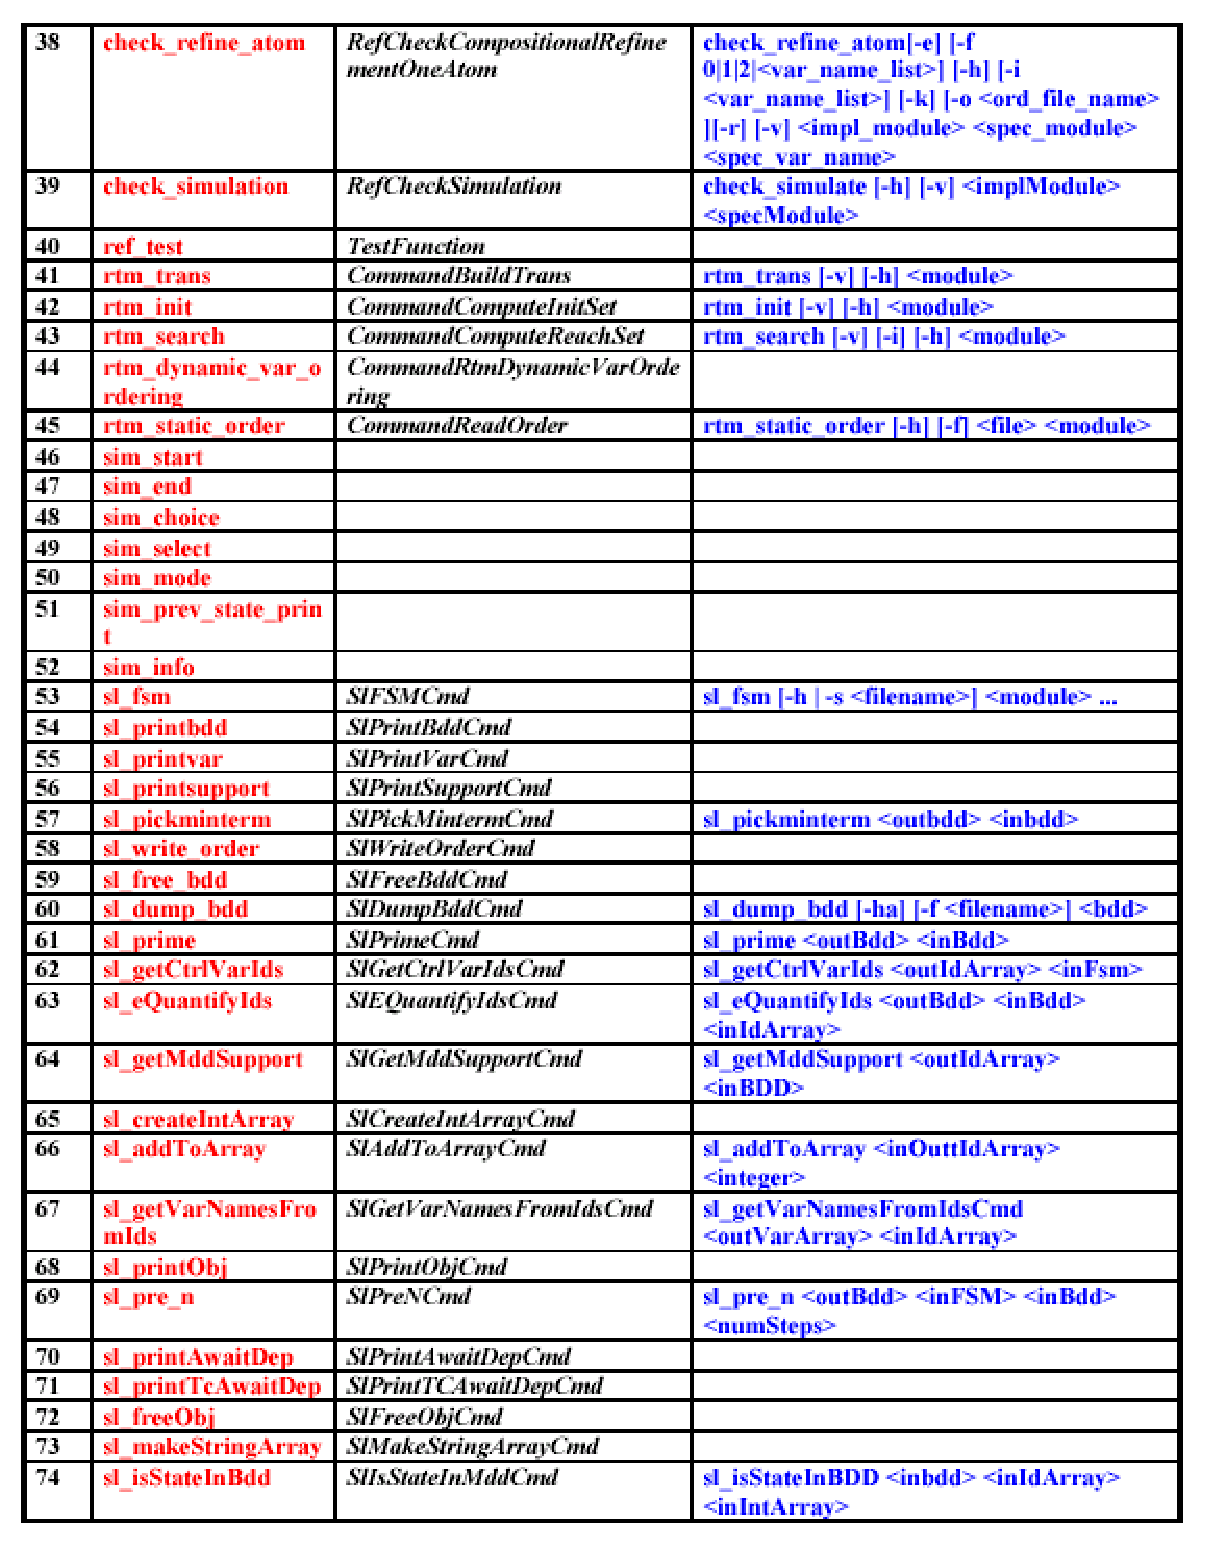
\includegraphics[width=5in]{figs/page-2}
%%\newpage
%%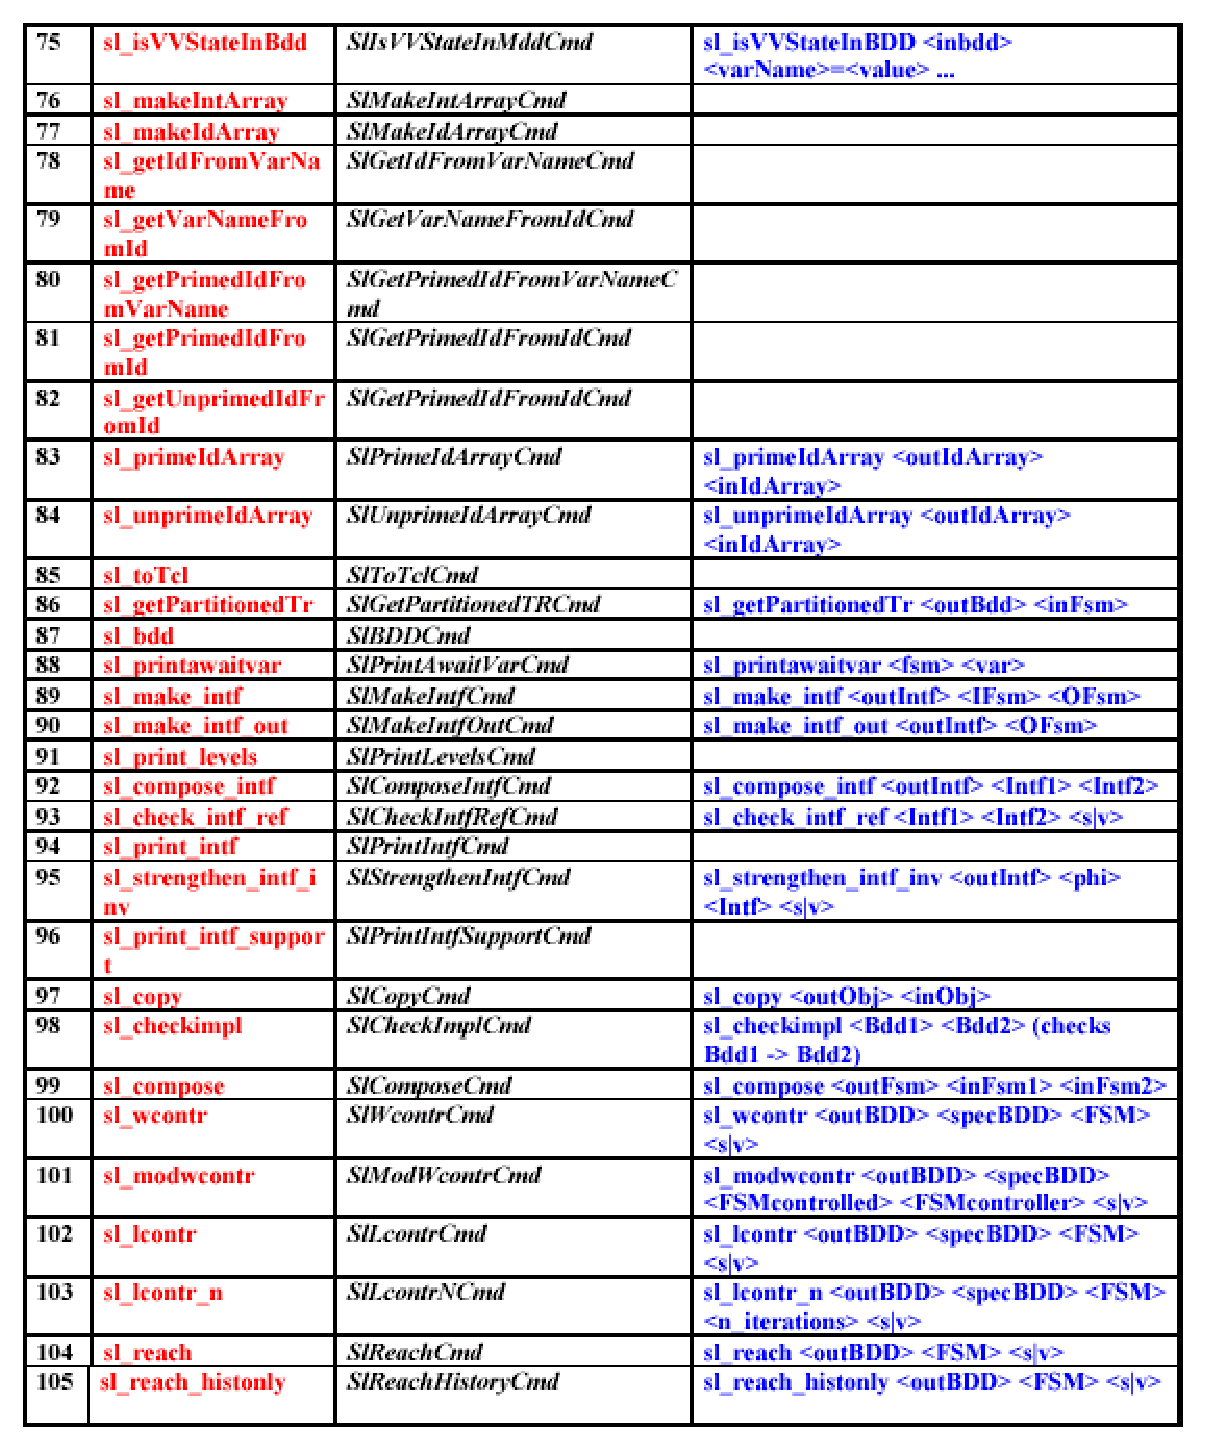
\includegraphics[width=5in]{figs/page-3}
%%\newpage
%%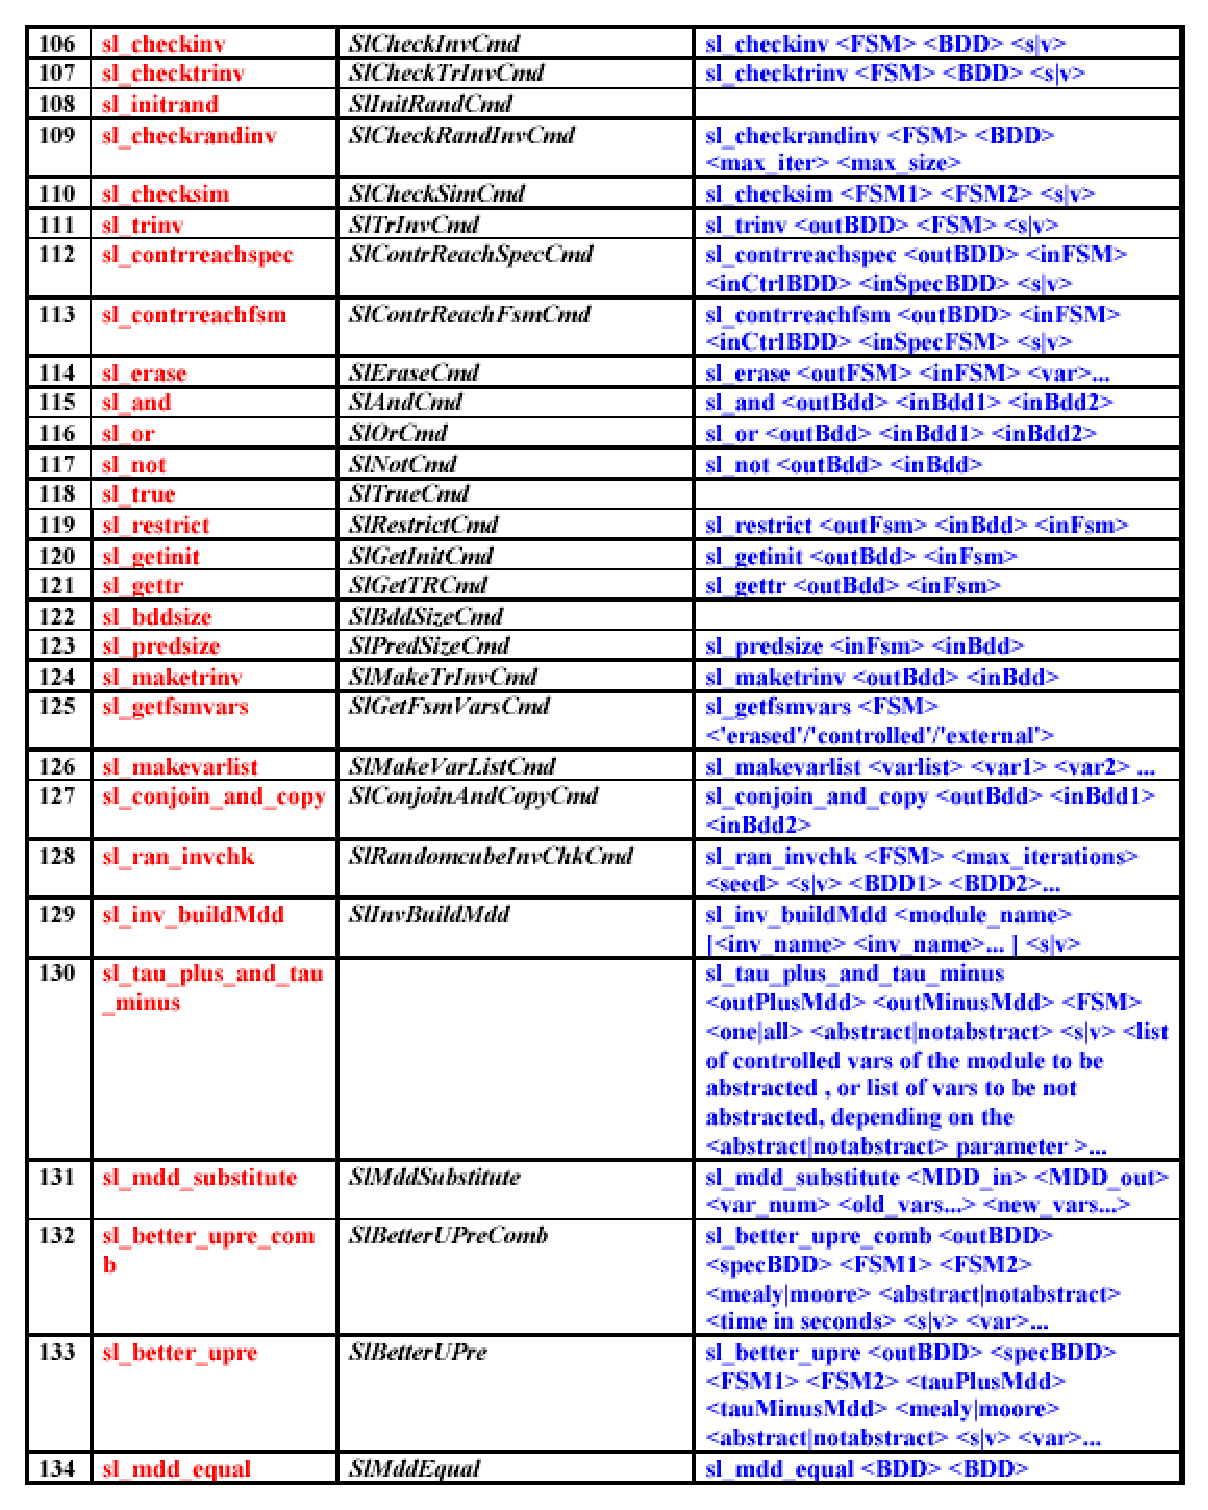
\includegraphics[width=5in]{figs/page-4}
%%\newpage
%%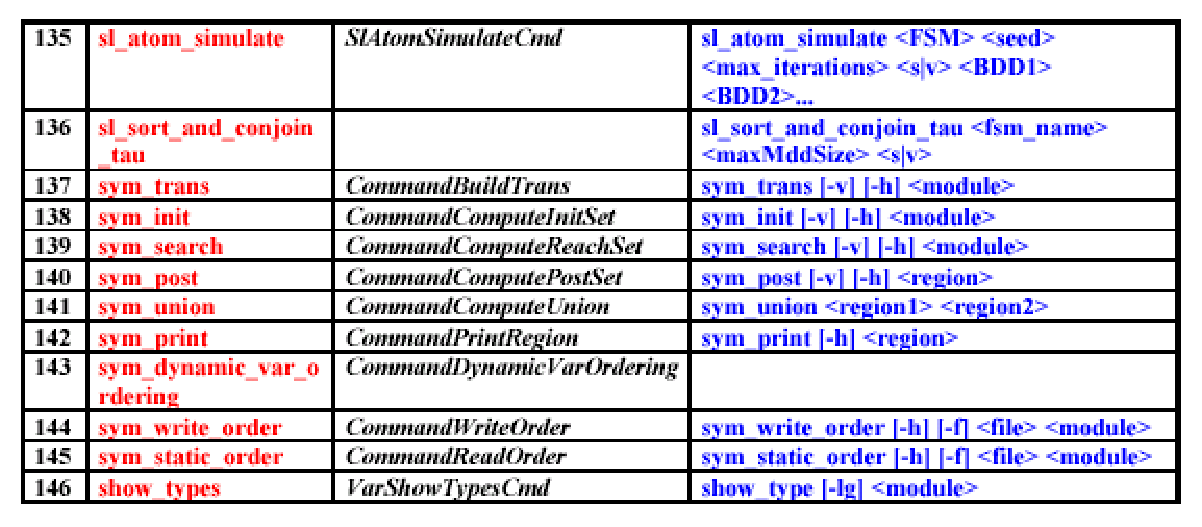
\includegraphics[width=5in]{figs/page-5}
%\caption{Chai Commands Summarized}
%\label{fig:chaicommands}
%\end{figure}
%
%\begin{longtable}{|l|l|l|}
%  \hline
%  % after \\: \hline or \cline{col1-col2} \cline{col3-col4} ...
%  SNo & Command & Function \\
%  \hline
% 1  &  atl\_read  &   \\
% \hline
% 2  &  atl\_print  &   \\
% \hline
% 3  &  \_atl\_convertToDag  &   \\
% \hline
% 4  &  enum\_init  &   ModuleComputeInitialSet \\
% \hline
% \multicolumn{3}{|l|} {Usage:  enum\_init [-h] $langle$module\_name$rangle$
%}\\
% \hline
% 5  &  enum\_post  &   StateComputePostSet \\
% \hline
% \multicolumn{3}{|l|} {Usage:  enum\_post [-h] $langle$state\_name$rangle$
%}\\
% \hline
% 6  &  state\_print  &   StatePrintVariableValues \\
% \hline
% \multicolumn{3}{|l|} {Usage:  state\_print [-h] $langle$state\_name$rangle$
%}\\
% \hline
% 7  &  enum\_search  &   ModulePerformEnumerativeSearch \\
% \hline
% \multicolumn{3}{|l|} {Usage:  enum\_search [-h] [-d] $langle$module\_name$rangle$
%}\\
% \hline
% 8  &  enum\_numVar  &   EnumNumVarCmd \\
% \hline
% 9  &  enum\_var  &   EnumVarCmd \\
% \hline
% 10  &  enum\_value  &   EnumValueCmd \\
% \hline
% 11  &  inv\_read  &   \\
% \hline
% 12  &  inv\_print  &   \\
% \hline
% 13  &  inv\_check  &   \\
% \hline
% 14  &  reinit  &   MochaReinitialize \\
% \hline
% 15  &  \_mocha\_end  &   MochaEnd \\
% \hline
% 16  &  atl\_check  &   \\
% \hline
% 17  &  show\_mdls  &   MdlShowModuleCmd \\
% \hline
% \multicolumn{3}{|l|} {Usage:  show\_mdls [haldg] [module]
%}\\
% \hline
% 18  &  save  &   MdlSaveCmd \\
% \hline
% 19  &  delete  &   MdlDeleteCmd \\
% \hline
% 20  &  show\_vars  &   MdlShowVariableCmd \\
% \hline
% \multicolumn{3}{|l|} {Usage:  show\_vars [-vHF|HD|EV|ALL] Module
%}\\
% \hline
% 21  &  compose  &   MdlComposeCmd \\
% \hline
% \multicolumn{3}{|l|} {Usage:  compose Module1 Module2
%}\\
% \hline
% 22  &  hide  &   MdlHideCmd \\
% \hline
% \multicolumn{3}{|l|} {Usage:  hide var1 var2 ...  Module
%}\\
% \hline
% 23  &  ren  &   MdlRenameCmd \\
% \hline
% \multicolumn{3}{|l|} {Usage:  ren from\_var to\_var Module
%}\\
% \hline
% 24  &  let  &   MdlLetCmd \\
% \hline
% \multicolumn{3}{|l|} {Usage:  let Module be Module1
%}\\
% \hline
% 25  &  isEventVariable  &   MdlIsEventVariableCmd \\
% \hline
% \multicolumn{3}{|l|} {Usage:  isEventVariable module variable
%}\\
% \hline
% 26  &  isPrivateVariable  &   MdlIsPrivateVariableCmd \\
% \hline
% \multicolumn{3}{|l|} {Usage:  isPrivateVariable module variable
%}\\
% \hline
% 27  &  isInterfaceVariable  &   MdlIsInterfaceVariableCmd \\
% \hline
% \multicolumn{3}{|l|} {Usage:  isInterfaceVariable module variable
%}\\
% \hline
% 28  &  isExternalVariable  &   MdlIsExternalVariableCmd \\
% \hline
% \multicolumn{3}{|l|} {Usage:  isExternalVariable module variable
%}\\
% \hline
% 29  &  isHistoryFree  &   MdlIsHistoryFreeCmd \\
% \hline
% \multicolumn{3}{|l|} {Usage:  isHistoryFree module variable
%}\\
% \hline
% 30  &  isModuleUpdate  &   MdlIsModuleUpdateCmd \\
% \hline
% 31  &  updateModule  &   MdlUpdateModuleCmd \\
% \hline
% 32  &  show\_atoms  &   MdlShowAtomsCmd \\
% \hline
% \multicolumn{3}{|l|} {Usage:  show\_atoms module
%}\\
% \hline
% 33  &  show\_components  &   \_MdlShowComponents \\
% \hline
% 34  &  traverse  &   MdlTraverseCmd \\
% \hline
% 35  &  read\_module  &   PrsReadModuleCmd \\
% \hline
% \multicolumn{3}{|l|} {Usage:  read\_module [-hp] $langle$filename$rangle$
%}\\
% \hline
% 36  &  read\_intf  &   PrsReadIntfCmd \\
% \hline
% \multicolumn{3}{|l|} {Usage:  read\_intf [-hp] $langle$filename$rangle$
%}\\
% \hline
% 37  &  check\_refine  &   RefCheckNohiddenRefinement \\
% \hline
% \multicolumn{3}{|l|} {Usage:  check\_refine [-h] [-o $langle$filename$rangle$] [-v]  $langle$implModule$rangle$ $langle$specModule$rangle$
%}\\
% \hline
% 38  &  check\_refine\_atom  &    RefCheckCompositionalRefinementOneAtom \\
% \hline
% \multicolumn{3}{|l|} {Usage:  check\_refine\_atom[-e]  [-f 0|1|2|$langle$var\_name\_list$rangle$] [-h] [-i $langle$var\_name\_list$rangle$] [-k]  [-o $langle$ord\_file\_name$rangle$ ][-r] [-v] $langle$impl\_module$rangle$ $langle$spec\_module$rangle$ $langle$spec\_var\_name$rangle$
%}\\
% \hline
% 39  &  check\_simulation  &    RefCheckSimulation \\
% \hline
% \multicolumn{3}{|l|} {Usage:  check\_simulate  [-h] [-v] $langle$implModule$rangle$ $langle$specModule$rangle$
%}\\
% \hline
% 40  &  ref\_test  &    TestFunction \\
% \hline
% 41  &  rtm\_trans  &   CommandBuildTrans \\
% \hline
% \multicolumn{3}{|l|} {Usage:  rtm\_trans [-v] [-h] $langle$module$rangle$
%}\\
% \hline
% 42  &  rtm\_init  &   CommandComputeInitSet \\
% \hline
% \multicolumn{3}{|l|} {Usage:  rtm\_init [-v] [-h] $langle$module$rangle$
%}\\
% \hline
% 43  &  rtm\_search  &   CommandComputeReachSet \\
% \hline
% \multicolumn{3}{|l|} {Usage:  rtm\_search [-v] [-i] [-h] $langle$module$rangle$
%}\\
% \hline
% 44  &  rtm\_dynamic\_var\_ordering  &   CommandRtmDynamicVarOrdering \\
% \hline
% 45  &  rtm\_static\_order  &   CommandReadOrder \\
% \hline
% \multicolumn{3}{|l|} {Usage:  rtm\_static\_order [-h] [-f] $langle$file$rangle$ $langle$module$rangle$
%}\\
% \hline
% 46  &  sim\_start  &   \\
% \hline
% 47  &  sim\_end  &   \\
% \hline
% 48  &  sim\_choice  &   \\
% \hline
% 49  &  sim\_select  &   \\
% \hline
% 50  &  sim\_mode  &   \\
% \hline
% 51  &  sim\_prev\_state\_print  &   \\
% \hline
% 52  &  sim\_info  &   \\
% \hline
% 53  &  sl\_fsm  &   SlFSMCmd \\
% \hline
% \multicolumn{3}{|l|} {Usage:  sl\_fsm [-h | -s $langle$filename$rangle$] $langle$module$rangle$ ...
%}\\
% \hline
% 54  &  sl\_printbdd  &   SlPrintBddCmd \\
% \hline
% 55  &  sl\_printvar  &   SlPrintVarCmd \\
% \hline
% 56  &  sl\_printsupport  &   SlPrintSupportCmd \\
% \hline
% 57  &  sl\_pickminterm  &   SlPickMintermCmd \\
% \hline
% \multicolumn{3}{|l|} {Usage:    sl\_pickminterm $langle$outbdd$rangle$ $langle$inbdd$rangle$
%}\\
% \hline
% 58  &  sl\_write\_order  &   SlWriteOrderCmd \\
% \hline
% 59  &  sl\_free\_bdd  &   SlFreeBddCmd \\
% \hline
% 60  &  sl\_dump\_bdd  &   SlDumpBddCmd \\
% \hline
% \multicolumn{3}{|l|} {Usage:  sl\_dump\_bdd [-ha] [-f $langle$filename$rangle$] $langle$bdd$rangle$
%}\\
% \hline
% 61  &  sl\_prime  &   SlPrimeCmd \\
% \hline
% \multicolumn{3}{|l|} {Usage:    sl\_prime $langle$outBdd$rangle$ $langle$inBdd$rangle$
%}\\
% \hline
% 62  &  sl\_getCtrlVarIds  &   SlGetCtrlVarIdsCmd \\
% \hline
% \multicolumn{3}{|l|} {Usage:    sl\_getCtrlVarIds $langle$outIdArray$rangle$ $langle$inFsm$rangle$
%}\\
% \hline
% 63  &  sl\_eQuantifyIds  &   SlEQuantifyIdsCmd \\
% \hline
% \multicolumn{3}{|l|} {Usage:    sl\_eQuantifyIds $langle$outBdd$rangle$ $langle$inBdd$rangle$ $langle$inIdArray$rangle$
%}\\
% \hline
% 64  &  sl\_getMddSupport  &   SlGetMddSupportCmd \\
% \hline
% \multicolumn{3}{|l|} {Usage:    sl\_getMddSupport $langle$outIdArray$rangle$ $langle$inBDD$rangle$
%}\\
% \hline
% 65  &  sl\_createIntArray  &   SlCreateIntArrayCmd \\
% \hline
% 66  &  sl\_addToArray  &   SlAddToArrayCmd \\
% \hline
% \multicolumn{3}{|l|} {Usage:    sl\_addToArray $langle$inOuttIdArray$rangle$ $langle$integer$rangle$
%}\\
% \hline
% 67  &  sl\_getVarNamesFromIds  &   SlGetVarNamesFromIdsCmd \\
% \hline
% \multicolumn{3}{|l|} {Usage:    sl\_getVarNamesFromIdsCmd $langle$outVarArray$rangle$ $langle$inIdArray$rangle$
%}\\
% \hline
% 68  &  sl\_printObj  &   SlPrintObjCmd \\
% \hline
% 69  &  sl\_pre\_n  &   SlPreNCmd \\
% \hline
% \multicolumn{3}{|l|} {Usage:    sl\_pre\_n $langle$outBdd$rangle$ $langle$inFSM$rangle$ $langle$inBdd$rangle$ $langle$numSteps$rangle$
%}\\
% \hline
% 70  &  sl\_printAwaitDep  &   SlPrintAwaitDepCmd \\
% \hline
% 71  &  sl\_printTcAwaitDep  &   SlPrintTCAwaitDepCmd \\
% \hline
% 72  &  sl\_freeObj  &   SlFreeObjCmd \\
% \hline
% 73  &  sl\_makeStringArray  &   SlMakeStringArrayCmd \\
% \hline
% 74  &  sl\_isStateInBdd  &   SlIsStateInMddCmd \\
% \hline
% \multicolumn{3}{|l|} {Usage:    sl\_isStateInBDD $langle$inbdd$rangle$ $langle$inIdArray$rangle$ $langle$inIntArray$rangle$
%}\\
% \hline
% 75  &  sl\_isVVStateInBdd  &   SlIsVVStateInMddCmd \\
% \hline
% \multicolumn{3}{|l|} {Usage:    sl\_isVVStateInBDD $langle$inbdd$rangle$ $langle$varName$rangle$=$langle$value$rangle$ ...
%}\\
% \hline
% 76  &  sl\_makeIntArray  &   SlMakeIntArrayCmd \\
% \hline
% 77  &  sl\_makeIdArray  &   SlMakeIdArrayCmd \\
% \hline
% 78  &  sl\_getIdFromVarName  &   SlGetIdFromVarNameCmd \\
% \hline
% 79  &  sl\_getVarNameFromId  &   SlGetVarNameFromIdCmd \\
% \hline
% 80  &  sl\_getPrimedIdFromVarName  &   SlGetPrimedIdFromVarNameCmd \\
% \hline
% 81  &  sl\_getPrimedIdFromId  &   SlGetPrimedIdFromIdCmd \\
% \hline
% 82  &  sl\_getUnprimedIdFromId  &   SlGetPrimedIdFromIdCmd \\
% \hline
% 83  &  sl\_primeIdArray  &   SlPrimeIdArrayCmd \\
% \hline
% \multicolumn{3}{|l|} {Usage:    sl\_primeIdArray $langle$outIdArray$rangle$ $langle$inIdArray$rangle$
%}\\
% \hline
% 84  &  sl\_unprimeIdArray  &   SlUnprimeIdArrayCmd \\
% \hline
% \multicolumn{3}{|l|} {Usage:    sl\_unprimeIdArray $langle$outIdArray$rangle$ $langle$inIdArray$rangle$
%}\\
% \hline
% 85  &  sl\_toTcl  &   SlToTclCmd \\
% \hline
% 86  &  sl\_getPartitionedTr  &   SlGetPartitionedTRCmd \\
% \hline
% \multicolumn{3}{|l|} {Usage:    sl\_getPartitionedTr $langle$outBdd$rangle$ $langle$inFsm$rangle$
%}\\
% \hline
% 87  &  sl\_bdd  &   SlBDDCmd \\
% \hline
% 88  &  sl\_printawaitvar  &   SlPrintAwaitVarCmd \\
% \hline
% \multicolumn{3}{|l|} {Usage:    sl\_printawaitvar $langle$fsm$rangle$ $langle$var$rangle$
%}\\
% \hline
% 89  &  sl\_make\_intf  &   SlMakeIntfCmd \\
% \hline
% \multicolumn{3}{|l|} {Usage:    sl\_make\_intf $langle$outIntf$rangle$ $langle$IFsm$rangle$ $langle$OFsm$rangle$
%}\\
% \hline
% 90  &  sl\_make\_intf\_out  &   SlMakeIntfOutCmd \\
% \hline
% \multicolumn{3}{|l|} {Usage:    sl\_make\_intf\_out $langle$outIntf$rangle$ $langle$OFsm$rangle$
%}\\
% \hline
% 91  &  sl\_print\_levels  &   SlPrintLevelsCmd \\
% \hline
% 92  &  sl\_compose\_intf  &   SlComposeIntfCmd \\
% \hline
% \multicolumn{3}{|l|} {Usage:    sl\_compose\_intf $langle$outIntf$rangle$ $langle$Intf1$rangle$ $langle$Intf2$rangle$
%}\\
% \hline
% 93  &  sl\_check\_intf\_ref  &   SlCheckIntfRefCmd \\
% \hline
% \multicolumn{3}{|l|} {Usage:    sl\_check\_intf\_ref $langle$Intf1$rangle$ $langle$Intf2$rangle$ $langle$s|v$rangle$
%}\\
% \hline
% 94  &  sl\_print\_intf  &   SlPrintIntfCmd \\
% \hline
% 95  &  sl\_strengthen\_intf\_inv  &   SlStrengthenIntfCmd \\
% \hline
% \multicolumn{3}{|l|} {Usage:    sl\_strengthen\_intf\_inv $langle$outIntf$rangle$ $langle$phi$rangle$ $langle$Intf$rangle$ $langle$s|v$rangle$
%}\\
% \hline
% 96  &  sl\_print\_intf\_support  &   SlPrintIntfSupportCmd \\
% \hline
% 97  &  sl\_copy  &   SlCopyCmd \\
% \hline
% \multicolumn{3}{|l|} {Usage:    sl\_copy $langle$outObj$rangle$ $langle$inObj$rangle$
%}\\
% \hline
% 98  &  sl\_checkimpl  &   SlCheckImplCmd \\
% \hline
% \multicolumn{3}{|l|} {Usage:    sl\_checkimpl $langle$Bdd1$rangle$ $langle$Bdd2$rangle$ (checks Bdd1 -$rangle$ Bdd2)
%}\\
% \hline
% 99  &  sl\_compose  &   SlComposeCmd \\
% \hline
% \multicolumn{3}{|l|} {Usage:    sl\_compose $langle$outFsm$rangle$ $langle$inFsm1$rangle$ $langle$inFsm2$rangle$
%}\\
% \hline
% 100  &  sl\_wcontr  &   SlWcontrCmd \\
% \hline
% \multicolumn{3}{|l|} {Usage:    sl\_wcontr $langle$outBDD$rangle$ $langle$specBDD$rangle$ $langle$FSM$rangle$ $langle$s|v$rangle$
%}\\
% \hline
% 101  &  sl\_modwcontr  &   SlModWcontrCmd \\
% \hline
% \multicolumn{3}{|l|} {Usage:    sl\_modwcontr $langle$outBDD$rangle$ $langle$specBDD$rangle$ $langle$FSMcontrolled$rangle$ $langle$FSMcontroller$rangle$ $langle$s|v$rangle$
%}\\
% \hline
% 102  &  sl\_lcontr  &   SlLcontrCmd \\
% \hline
% \multicolumn{3}{|l|} {Usage:    sl\_lcontr $langle$outBDD$rangle$ $langle$specBDD$rangle$ $langle$FSM$rangle$ $langle$s|v$rangle$
%}\\
% \hline
% 103  &  sl\_lcontr\_n  &   SlLcontrNCmd \\
% \hline
% \multicolumn{3}{|l|} {Usage:    sl\_lcontr\_n $langle$outBDD$rangle$ $langle$specBDD$rangle$ $langle$FSM$rangle$ $langle$n\_iterations$rangle$ $langle$s|v$rangle$
%}\\
% \hline
% 104  &  sl\_reach  &   SlReachCmd \\
% \hline
% \multicolumn{3}{|l|} {Usage:    sl\_reach $langle$outBDD$rangle$ $langle$FSM$rangle$ $langle$s|v$rangle$
%}\\
% \hline
% 105  &  sl\_reach\_histonly  &   SlReachHistoryCmd \\
% \hline
% \multicolumn{3}{|l|} {Usage:    sl\_reach\_histonly $langle$outBDD$rangle$ $langle$FSM$rangle$ $langle$s|v$rangle$
%}\\
% \hline
% 106  &  sl\_checkinv  &   SlCheckInvCmd \\
% \hline
% \multicolumn{3}{|l|} {Usage:    sl\_checkinv $langle$FSM$rangle$ $langle$BDD$rangle$ $langle$s|v$rangle$
%}\\
% \hline
% 107  &  sl\_checktrinv  &   SlCheckTrInvCmd \\
% \hline
% \multicolumn{3}{|l|} {Usage:    sl\_checktrinv $langle$FSM$rangle$ $langle$BDD$rangle$ $langle$s|v$rangle$
%}\\
% \hline
% 108  &  sl\_initrand  &   SlInitRandCmd \\
% \hline
% 109  &  sl\_checkrandinv  &   SlCheckRandInvCmd \\
% \hline
% \multicolumn{3}{|l|} {Usage:  sl\_checkrandinv $langle$FSM$rangle$ $langle$BDD$rangle$ $langle$max\_iter$rangle$ $langle$max\_size$rangle$
%}\\
% \hline
% 110  &  sl\_checksim  &   SlCheckSimCmd \\
% \hline
% \multicolumn{3}{|l|} {Usage:    sl\_checksim $langle$FSM1$rangle$ $langle$FSM2$rangle$ $langle$s|v$rangle$
%}\\
% \hline
% 111  &  sl\_trinv  &   SlTrInvCmd \\
% \hline
% \multicolumn{3}{|l|} {Usage:    sl\_trinv $langle$outBDD$rangle$ $langle$FSM$rangle$ $langle$s|v$rangle$
%}\\
% \hline
% 112  &  sl\_contrreachspec  &   SlContrReachSpecCmd \\
% \hline
% \multicolumn{3}{|l|} {Usage:    sl\_contrreachspec $langle$outBDD$rangle$ $langle$inFSM$rangle$ $langle$inCtrlBDD$rangle$ $langle$inSpecBDD$rangle$ $langle$s|v$rangle$
%}\\
% \hline
% 113  &  sl\_contrreachfsm  &   SlContrReachFsmCmd \\
% \hline
% \multicolumn{3}{|l|} {Usage:    sl\_contrreachfsm $langle$outBDD$rangle$ $langle$inFSM$rangle$ $langle$inCtrlBDD$rangle$ $langle$inSpecFSM$rangle$ $langle$s|v$rangle$
%}\\
% \hline
% 114  &  sl\_erase  &   SlEraseCmd \\
% \hline
% \multicolumn{3}{|l|} {Usage:    sl\_erase $langle$outFSM$rangle$ $langle$inFSM$rangle$ $langle$var$rangle$...
%}\\
% \hline
% 115  &  sl\_and  &   SlAndCmd \\
% \hline
% \multicolumn{3}{|l|} {Usage:    sl\_and $langle$outBdd$rangle$ $langle$inBdd1$rangle$ $langle$inBdd2$rangle$
%}\\
% \hline
% 116  &  sl\_or  &   SlOrCmd \\
% \hline
% \multicolumn{3}{|l|} {Usage:    sl\_or $langle$outBdd$rangle$ $langle$inBdd1$rangle$ $langle$inBdd2$rangle$
%}\\
% \hline
% 117  &  sl\_not  &   SlNotCmd \\
% \hline
% \multicolumn{3}{|l|} {Usage:    sl\_not $langle$outBdd$rangle$ $langle$inBdd$rangle$
%}\\
% \hline
% 118  &  sl\_true  &   SlTrueCmd \\
% \hline
% 119  &  sl\_restrict  &   SlRestrictCmd \\
% \hline
% \multicolumn{3}{|l|} {Usage:    sl\_restrict $langle$outFsm$rangle$ $langle$inBdd$rangle$ $langle$inFsm$rangle$
%}\\
% \hline
% 120  &  sl\_getinit  &   SlGetInitCmd \\
% \hline
% \multicolumn{3}{|l|} {Usage:    sl\_getinit $langle$outBdd$rangle$ $langle$inFsm$rangle$
%}\\
% \hline
% 121  &  sl\_gettr  &   SlGetTRCmd \\
% \hline
% \multicolumn{3}{|l|} {Usage:    sl\_gettr $langle$outBdd$rangle$ $langle$inFsm$rangle$
%}\\
% \hline
% 122  &  sl\_bddsize  &   SlBddSizeCmd \\
% \hline
% 123  &  sl\_predsize  &   SlPredSizeCmd \\
% \hline
% \multicolumn{3}{|l|} {Usage:    sl\_predsize $langle$inFsm$rangle$ $langle$inBdd$rangle$
%}\\
% \hline
% 124  &  sl\_maketrinv  &   SlMakeTrInvCmd \\
% \hline
% \multicolumn{3}{|l|} {Usage:    sl\_maketrinv $langle$outBdd$rangle$ $langle$inBdd$rangle$
%}\\
% \hline
% 125  &  sl\_getfsmvars  &   SlGetFsmVarsCmd \\
% \hline
% \multicolumn{3}{|l|} {Usage:    sl\_getfsmvars $langle$FSM$rangle$ $langle$'erased'/'controlled'/'external'$rangle$
%}\\
% \hline
% 126  &  sl\_makevarlist  &   SlMakeVarListCmd \\
% \hline
% \multicolumn{3}{|l|} {Usage:    sl\_makevarlist $langle$varlist$rangle$ $langle$var1$rangle$ $langle$var2$rangle$ ...
%}\\
% \hline
% 127  &  sl\_conjoin\_and\_copy  &   SlConjoinAndCopyCmd \\
% \hline
% \multicolumn{3}{|l|} {Usage:    sl\_conjoin\_and\_copy $langle$outBdd$rangle$ $langle$inBdd1$rangle$ $langle$inBdd2$rangle$
%}\\
% \hline
% 128  &  sl\_ran\_invchk  &   SlRandomcubeInvChkCmd \\
% \hline
% \multicolumn{3}{|l|} {Usage:    sl\_ran\_invchk $langle$FSM$rangle$ $langle$max\_iterations$rangle$ $langle$seed$rangle$ $langle$s|v$rangle$ $langle$BDD1$rangle$ $langle$BDD2$rangle$...
%}\\
% \hline
% 129  &  sl\_inv\_buildMdd  &   SlInvBuildMdd \\
% \hline
% \multicolumn{3}{|l|} {Usage:    sl\_inv\_buildMdd $langle$module\_name$rangle$ [$langle$inv\_name$rangle$ $langle$inv\_name$rangle$... ] $langle$s|v$rangle$
%}\\
% \hline
% 130  &  sl\_tau\_plus\_and\_tau\_minus  &    \\
% \hline
% \multicolumn{3}{|l|} {Usage:    sl\_tau\_plus\_and\_tau\_minus $langle$outPlusMdd$rangle$ $langle$outMinusMdd$rangle$ $langle$FSM$rangle$ $langle$one|all$rangle$ $langle$abstract|notabstract$rangle$ $langle$s|v$rangle$ $langle$list of controlled vars of the module to be abstracted , or list of vars to be not abstracted, depending on the $langle$abstract|notabstract$rangle$ parameter $rangle$...
%}\\
% \hline
% 131  &  sl\_mdd\_substitute  &   SlMddSubstitute \\
% \hline
% \multicolumn{3}{|l|} {Usage:    sl\_mdd\_substitute $langle$MDD\_in$rangle$ $langle$MDD\_out$rangle$ $langle$var\_num$rangle$ $langle$old\_vars...$rangle$ $langle$new\_vars...$rangle$
%}\\
% \hline
% 132  &  sl\_better\_upre\_comb  &   SlBetterUPreComb \\
% \hline
% \multicolumn{3}{|l|} {Usage:    sl\_better\_upre\_comb $langle$outBDD$rangle$ $langle$specBDD$rangle$ $langle$FSM1$rangle$ $langle$FSM2$rangle$ $langle$maxTauSize$rangle$ $langle$mealy|moore$rangle$ $langle$abstract|notabstract$rangle$ $langle$time in seconds$rangle$ $langle$s|v$rangle$  $langle$var$rangle$...
%}\\
% \hline
% 133  &  sl\_better\_upre  &   SlBetterUPre \\
% \hline
% \multicolumn{3}{|l|} {Usage:    sl\_better\_upre $langle$outBDD$rangle$ $langle$specBDD$rangle$ $langle$FSM1$rangle$ $langle$FSM2$rangle$ $langle$tauPlusMdd$rangle$ $langle$tauMinusMdd$rangle$ $langle$mealy|moore$rangle$ $langle$abstract|notabstract$rangle$ $langle$s|v$rangle$  $langle$var$rangle$...
%}\\
% \hline
% 134  &  sl\_mdd\_equal  &   SlMddEqual \\
% \hline
% \multicolumn{3}{|l|} {Usage:    sl\_mdd\_equal $langle$BDD$rangle$ $langle$BDD$rangle$
%}\\
% \hline
% 135  &  sl\_atom\_simulate  &   SlAtomSimulateCmd \\
% \hline
% \multicolumn{3}{|l|} {Usage:    sl\_atom\_simulate $langle$FSM$rangle$  $langle$seed$rangle$ $langle$max\_iterations$rangle$ $langle$s|v$rangle$ $langle$BDD1$rangle$ $langle$BDD2$rangle$...
%}\\
% \hline
% 136  &  sl\_tbl\_lookup\_sim  &   SlTblLookupSimCmd \\
% \hline
% \multicolumn{3}{|l|} {Usage:    sl\_tbl\_lookup\_sim $langle$FSM$rangle$  $langle$seed$rangle$ $langle$max\_iterations$rangle$ $langle$s|v$rangle$ $langle$BDD1$rangle$ $langle$BDD2$rangle$...
%}\\
% \hline
% 137  &  sl\_checkinv\_abs  &   SlCheckInvAbsCmd \\
% \hline
% 138  &  sl\_counter\_eg\_refine  &   SlCounterEgRefineCmd \\
% \hline
% 139  &  sym\_trans  &   CommandBuildTrans \\
% \hline
% \multicolumn{3}{|l|} {Usage:  sym\_trans [-v] [-h] $langle$module$rangle$
%}\\
% \hline
% 140  &  sym\_init  &   CommandComputeInitSet \\
% \hline
% \multicolumn{3}{|l|} {Usage:  sym\_init [-v] [-h] $langle$module$rangle$
%}\\
% \hline
% 141  &  sym\_search  &   CommandComputeReachSet \\
% \hline
% \multicolumn{3}{|l|} {Usage:  sym\_search [-v] [-h] $langle$module$rangle$
%}\\
% \hline
% 142  &  sym\_post  &   CommandComputePostSet \\
% \hline
% \multicolumn{3}{|l|} {Usage:  sym\_post [-v] [-h] $langle$region$rangle$
%}\\
% \hline
% 143  &  sym\_union  &   CommandComputeUnion \\
% \hline
% \multicolumn{3}{|l|} {Usage:  sym\_union $langle$region1$rangle$ $langle$region2$rangle$
%}\\
% \hline
% 144  &  sym\_print  &   CommandPrintRegion \\
% \hline
% \multicolumn{3}{|l|} {Usage:  sym\_print [-h] $langle$region$rangle$
%}\\
% \hline
% 145  &  sym\_dynamic\_var\_ordering  &   CommandDynamicVarOrdering \\
% \hline
% 146  &  sym\_write\_order  &   CommandWriteOrder \\
% \hline
% \multicolumn{3}{|l|} {Usage:  sym\_write\_order [-h] [-f] $langle$file$rangle$ $langle$module$rangle$
%}\\
% \hline
% 147  &  sym\_static\_order  &   CommandReadOrder \\
% \hline
% \multicolumn{3}{|l|} {Usage:  sym\_static\_order [-h] [-f] $langle$file$rangle$ $langle$module$rangle$
%}\\
% \hline
% 148  &  show\_types  &   VarShowTypesCmd \\
% \hline
% \multicolumn{3}{|l|} {Usage:  show\_type [-lg] $langle$module$rangle$
%}\\
% \hline
%\end{longtable}
